\documentclass[12pt,a4paper]{report}

% Packages
\usepackage[utf8]{inputenc}
\usepackage[T1]{fontenc}
\usepackage{geometry}
\usepackage{graphicx}
\usepackage{amsmath}
\usepackage{amssymb}
\usepackage{fancyhdr}
\usepackage{titlesec}
\usepackage{tocloft}
\usepackage{hyperref}
\usepackage{listings}
\usepackage{xcolor}
\usepackage{tikz}
\usetikzlibrary{arrows, positioning, shapes, fit}
\usepackage{float}
\usepackage{caption}
\usepackage{subcaption}
\usepackage{enumitem}
\usepackage{longtable}
\usepackage{booktabs}
\usepackage{array}
\usepackage{multirow}
\usepackage{pdflscape}
\usepackage{afterpage}

% Page setup
\geometry{a4paper, margin=1in}
\setlength{\headheight}{15pt}

% Header and footer
\pagestyle{fancy}
\fancyhf{}
\fancyhead[L]{Campus-Sync Report}
\fancyhead[R]{B.Tech Project Exhibition 2024-2025}
\fancyfoot[C]{\leftmark}

\title{Compact Diagram Test}
\author{Campus-Sync Team}

\begin{document}

\chapter{Compact Diagram Test}

\section{Authentication Workflow}

\begin{figure}[H]
    \centering
    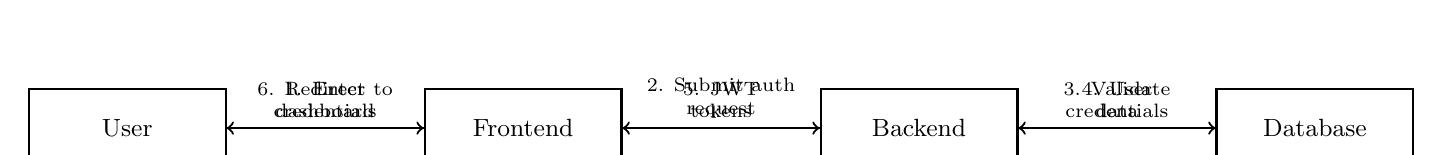
\begin{tikzpicture}[thick, node distance=2.5cm, every node/.style={align=center, font=\small}]
        \node (user) [draw, rectangle, minimum width=2.5cm, minimum height=1cm] {User};
        \node (frontend) [draw, rectangle, minimum width=2.5cm, minimum height=1cm, right=of user] {Frontend};
        \node (backend) [draw, rectangle, minimum width=2.5cm, minimum height=1cm, right=of frontend] {Backend};
        \node (database) [draw, rectangle, minimum width=2.5cm, minimum height=1cm, right=of backend] {Database};
        
        \draw[->] (user) -- (frontend) node[midway, above, font=\scriptsize] {1. Enter\\credentials};
        \draw[->] (frontend) -- (backend) node[midway, above, font=\scriptsize] {2. Submit auth\\request};
        \draw[->] (backend) -- (database) node[midway, above, font=\scriptsize] {3. Validate\\credentials};
        \draw[->] (database) -- (backend) node[midway, above, font=\scriptsize] {4. User\\data};
        \draw[->] (backend) -- (frontend) node[midway, above, font=\scriptsize] {5. JWT\\tokens};
        \draw[->] (frontend) -- (user) node[midway, above, font=\scriptsize] {6. Redirect to\\dashboard};
    \end{tikzpicture}
    \caption{Authentication Flow}
    \label{fig:auth-flow}
\end{figure}

\section{Assignment Submission Process}

\begin{figure}[H]
    \centering
    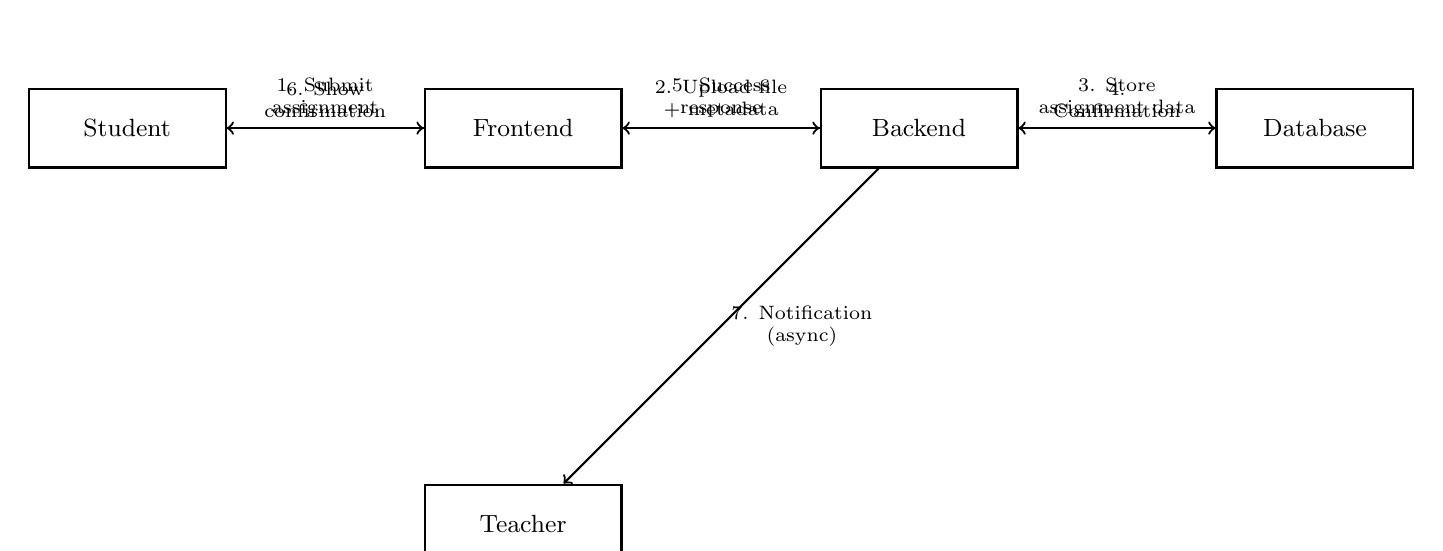
\begin{tikzpicture}[thick, node distance=2.5cm, every node/.style={align=center, font=\small}]
        \node (student) [draw, rectangle, minimum width=2.5cm, minimum height=1cm] {Student};
        \node (frontend) [draw, rectangle, minimum width=2.5cm, minimum height=1cm, right=of student] {Frontend};
        \node (backend) [draw, rectangle, minimum width=2.5cm, minimum height=1cm, right=of frontend] {Backend};
        \node (database) [draw, rectangle, minimum width=2.5cm, minimum height=1cm, right=of backend] {Database};
        \node (teacher) [draw, rectangle, minimum width=2.5cm, minimum height=1cm, below=of frontend, yshift=-1.5cm] {Teacher};
        
        \draw[->] (student) -- (frontend) node[midway, above, font=\scriptsize] {1. Submit\\assignment};
        \draw[->] (frontend) -- (backend) node[midway, above, font=\scriptsize] {2. Upload file\\+ metadata};
        \draw[->] (backend) -- (database) node[midway, above, font=\scriptsize] {3. Store\\assignment data};
        \draw[->] (database) -- (backend) node[midway, above, font=\scriptsize] {4.\\Confirmation};
        \draw[->] (backend) -- (frontend) node[midway, above, font=\scriptsize] {5. Success\\response};
        \draw[->] (frontend) -- (student) node[midway, above, font=\scriptsize] {6. Show\\confirmation};
        \draw[->] (backend) -- (teacher) node[midway, right, font=\scriptsize] {7. Notification\\(async)};
    \end{tikzpicture}
    \caption{Assignment Submission Flow}
    \label{fig:assignment-flow}
\end{figure}

\section{Component Hierarchy}

\begin{figure}[H]
    \centering
    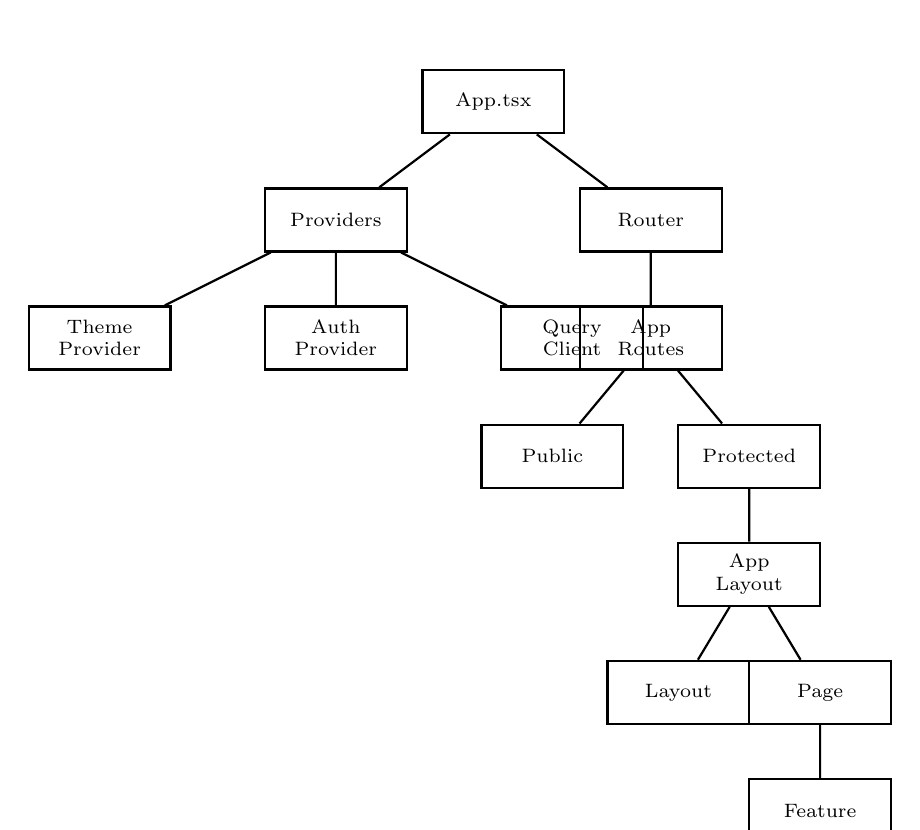
\begin{tikzpicture}[thick, level distance=1.5cm,
      level 1/.style={sibling distance=4cm},
      level 2/.style={sibling distance=3cm},
      level 3/.style={sibling distance=2.5cm},
      level 4/.style={sibling distance=2cm},
      level 5/.style={sibling distance=1.8cm},
      level 6/.style={sibling distance=1.5cm},
      every node/.style={align=center, rectangle, draw, minimum width=1.8cm, minimum height=0.8cm, font=\scriptsize}]
      \node {App.tsx}
        child { node {Providers}
          child { node {Theme\\Provider} }
          child { node {Auth\\Provider} }
          child { node {Query\\Client} }
        }
        child { node {Router}
          child { node {App\\Routes}
            child { node {Public} }
            child { node {Protected}
              child { node {App\\Layout}
                child { node {Layout} }
                child { node {Page}
                  child { node {Feature} }
                }
              }
            }
          }
        };
    \end{tikzpicture}
    \caption{Component Hierarchy Tree}
    \label{fig:component-hierarchy}
\end{figure}

\end{document}